\documentclass{standalone}
\usepackage{tikz}
\usepackage{ctex,siunitx}
\setCJKmainfont{Noto Serif CJK SC}
\usepackage{tkz-euclide}
\usepackage{amsmath}
\usetikzlibrary{patterns, calc}
\usetikzlibrary {decorations.pathmorphing, decorations.pathreplacing, decorations.shapes,}

\begin{document}
\small
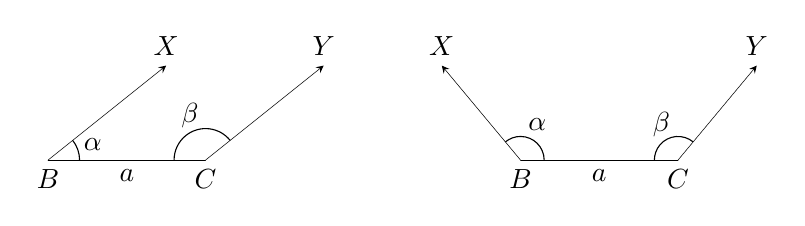
\begin{tikzpicture}[>=stealth,scale=1]
  \tkzSetUpPoint[fill=black]
  % \useasboundingbox(-1,-0.75)rectangle(3.7,1.4);
  \begin{scope}
    \tkzDefPoints{0/0/B, 2/0/C, 1.5/1.2/X, 3.5/1.2/Y}
  \tkzDrawSegments[->](B,X C,Y)
  \tkzDrawSegments(B,C)
  \tkzLabelSegment[below](B,C){$a$}
  \tkzLabelPoints[below](B,C)
  \tkzLabelPoints[above](X,Y)
  \tkzMarkAngles[mark=none,size=.4](C,B,X Y,C,B)
  \tkzLabelAngle[pos=.6](C,B,X){$\alpha$}
  \tkzLabelAngle[pos=.6](Y,C,B){$\beta$}
  \end{scope}
  \begin{scope}[xshift=6cm]
    \tkzDefPoints{0/0/B, 2/0/C, -1/1.2/X, 3/1.2/Y}
    \tkzDrawSegments[->](B,X C,Y)
    \tkzDrawSegments(B,C)
    \tkzLabelSegment[below](B,C){$a$}
    \tkzLabelPoints[below](B,C)
    \tkzLabelPoints[above](X,Y)
    \tkzMarkAngles[mark=none,size=.3](C,B,X Y,C,B)
    \tkzLabelAngle[pos=.5](C,B,X){$\alpha$}
    \tkzLabelAngle[pos=.5](Y,C,B){$\beta$}
  \end{scope}
\end{tikzpicture}
\end{document}